\documentclass[11pt,a4paper]{article}

\usepackage[margin=1in]{geometry}
\usepackage{booktabs}
\usepackage{graphicx}
\usepackage{array}
\usepackage{enumitem}
\usepackage{hyperref}
\usepackage{xcolor}
\usepackage{amsmath,amssymb}
\usepackage{caption}
\usepackage{subcaption}

\hypersetup{
    colorlinks=true,
    linkcolor=blue!50!black,
    citecolor=blue!50!black,
    urlcolor=blue!50!black
}

\setlist{itemsep=2pt,topsep=4pt}
\renewcommand{\arraystretch}{1.2}

\title{
    \textbf{PakAgriVision: Crop Disease Detector}\\
    \large Deliverable 1: Problem Definition \& Data Foundations\\
    \normalsize Track A: Application Development
}

\author{
    \textbf{Abdul Ahad} (24L-3029) \quad 
    \textbf{M. Anas} (24L-3004) \quad 
    \textbf{M. Babar Shahzad} (24L-3047)\\[4pt]
    \small National University of Computer and Emerging Sciences (FAST-NUCES)\\
    \small Repository: \url{https://github.com/ErenYeagerJinko/PakAgriVision}
}

\date{\today}

\begin{document}

\maketitle

\begin{abstract}
PakAgriVision is an AI-driven agricultural decision-support tool addressing late crop disease detection for Pakistani smallholder farmers. This report presents Deliverable~1, establishing the problem definition, raw data foundations from the PlantVillage benchmark ($\sim$54,000 images across 38 classes), local field image metadata collection, data validation and deduplication protocols, stratified leakage-free split strategies, and a standardized 13-field treatment knowledge base schema.
\end{abstract}

\section{Problem Statement \& Objectives}
\label{sec:problem}

\subsection{Agricultural Context in Pakistan}
Agriculture forms the backbone of Pakistan's economy, employing over 37\% of the labor force and contributing roughly 23\% of GDP. However, smallholder farmers experience substantial post-harvest and crop yield losses (often between 20\% to 40\%) due to preventable fungal, bacterial, and viral foliar diseases in staple crops including tomato, potato, apple, and corn. Traditional diagnosis relies on infrequent visits from agricultural extension officers, leading to late or erroneous pesticide interventions.

\subsection{Project Vision: PakAgriVision}
PakAgriVision is an accessible, web-based diagnostic application that bridges this gap. When a farmer or field worker uploads a smartphone image of a symptomatic leaf, the system provides:
\begin{enumerate}
    \item \textbf{Disease Classification:} Identification across 38 crop-condition classes with top-1 and top-3 confidence scores.
    \item \textbf{Visual Interpretability (Grad-CAM):} Heatmap overlays identifying the specific anatomical regions of the leaf informing the classification.
    \item \textbf{Actionable Treatment Engine:} Structured, bilingual (English and Urdu) advisory covering chemical controls, organic alternatives, dosage recommendations, and preventative farming practices.
\end{enumerate}

\section{Dataset Acquisition \& Provenance}
\label{sec:dataset}

\subsection{PlantVillage Benchmark Dataset}
The primary baseline training dataset is the public PlantVillage benchmark~\cite{plantvillage}, obtained via the Kaggle API (\texttt{abdallahalidev/plantvillage-dataset}).
\begin{itemize}
    \item \textbf{Total Scale:} 54,303 color images across 14 distinct crop species and 38 distinct crop-disease pairings.
    \item \textbf{Input Resolution:} Standardized 256$\times$256 pixels in RGB color format.
    \item \textbf{License \& Integrity:} CC0 Public Domain / Open Educational License.
\end{itemize}

\subsection{Field-Image Collection for Domain Shift Evaluation}
Because standard PlantVillage images were captured under controlled laboratory lighting against monochrome gray/black backgrounds, models trained naively exhibit brittle performance when deployed in field conditions. To rigorously assess generalization, PakAgriVision incorporates a dedicated field-collected test set ($\ge$150 images) documenting leaves under natural Pakistani sunlight, soil backgrounds, and complex foliage occlusion. Metadata, sources, and crop-name mappings are tracked in \texttt{field\_meta/field\_labels.csv} and \texttt{field\_meta/class\_mapping.csv}.

\section{Data Verification \& Quality Assurance}
\label{sec:cleaning}

Prior to partitioning and training, raw data undergoes automated verification through \texttt{data\_scripts/}:
\begin{itemize}
    \item \textbf{File Integrity Verification:} Binary validation via Pillow (\texttt{PIL.Image.verify()}) to catch truncated JPEG files and corrupt headers.
    \item \textbf{Dimension \& Channel Consistency:} Enforcing 3-channel RGB representation and discarding monochrome or non-standard color modes.
    \item \textbf{Deduplication via Perceptual Hashing:} Computing Difference Hashes (dHash) and Average Hashes (aHash) with \texttt{imagehash} at a Hamming distance threshold $\le 2$ to identify near-identical image duplicates across partitions, preventing data leakage.
\end{itemize}
The output log and identified duplicates are archived into \texttt{splits/dedupe\_report.csv}.

\section{Exploratory Data Analysis (EDA)}
\label{sec:eda}

Exploratory analysis was conducted in \texttt{notebooks/01\_eda.ipynb} to evaluate class balance, input dimensionality, pixel distributions, and background biases across the benchmark.

\subsection{Class Distribution and Imbalance}
The curated dataset comprises 38 crop-disease classes across 14 plant species totaling 31,694 images. Prior to curation, the raw dataset exhibited extreme imbalance (a 36.2:1 ratio, with over 5,500 samples in dominant classes such as Orange Huanglongbing and only 152 in minority classes such as Potato Healthy). Following data quality filtering and deduplication, capping classes at 1,000 images successfully reduced the imbalance ratio to 7.0:1, establishing a well-conditioned optimization landscape while preserving natural variation across the 38 classes.

\begin{figure}[htbp]
    \centering
    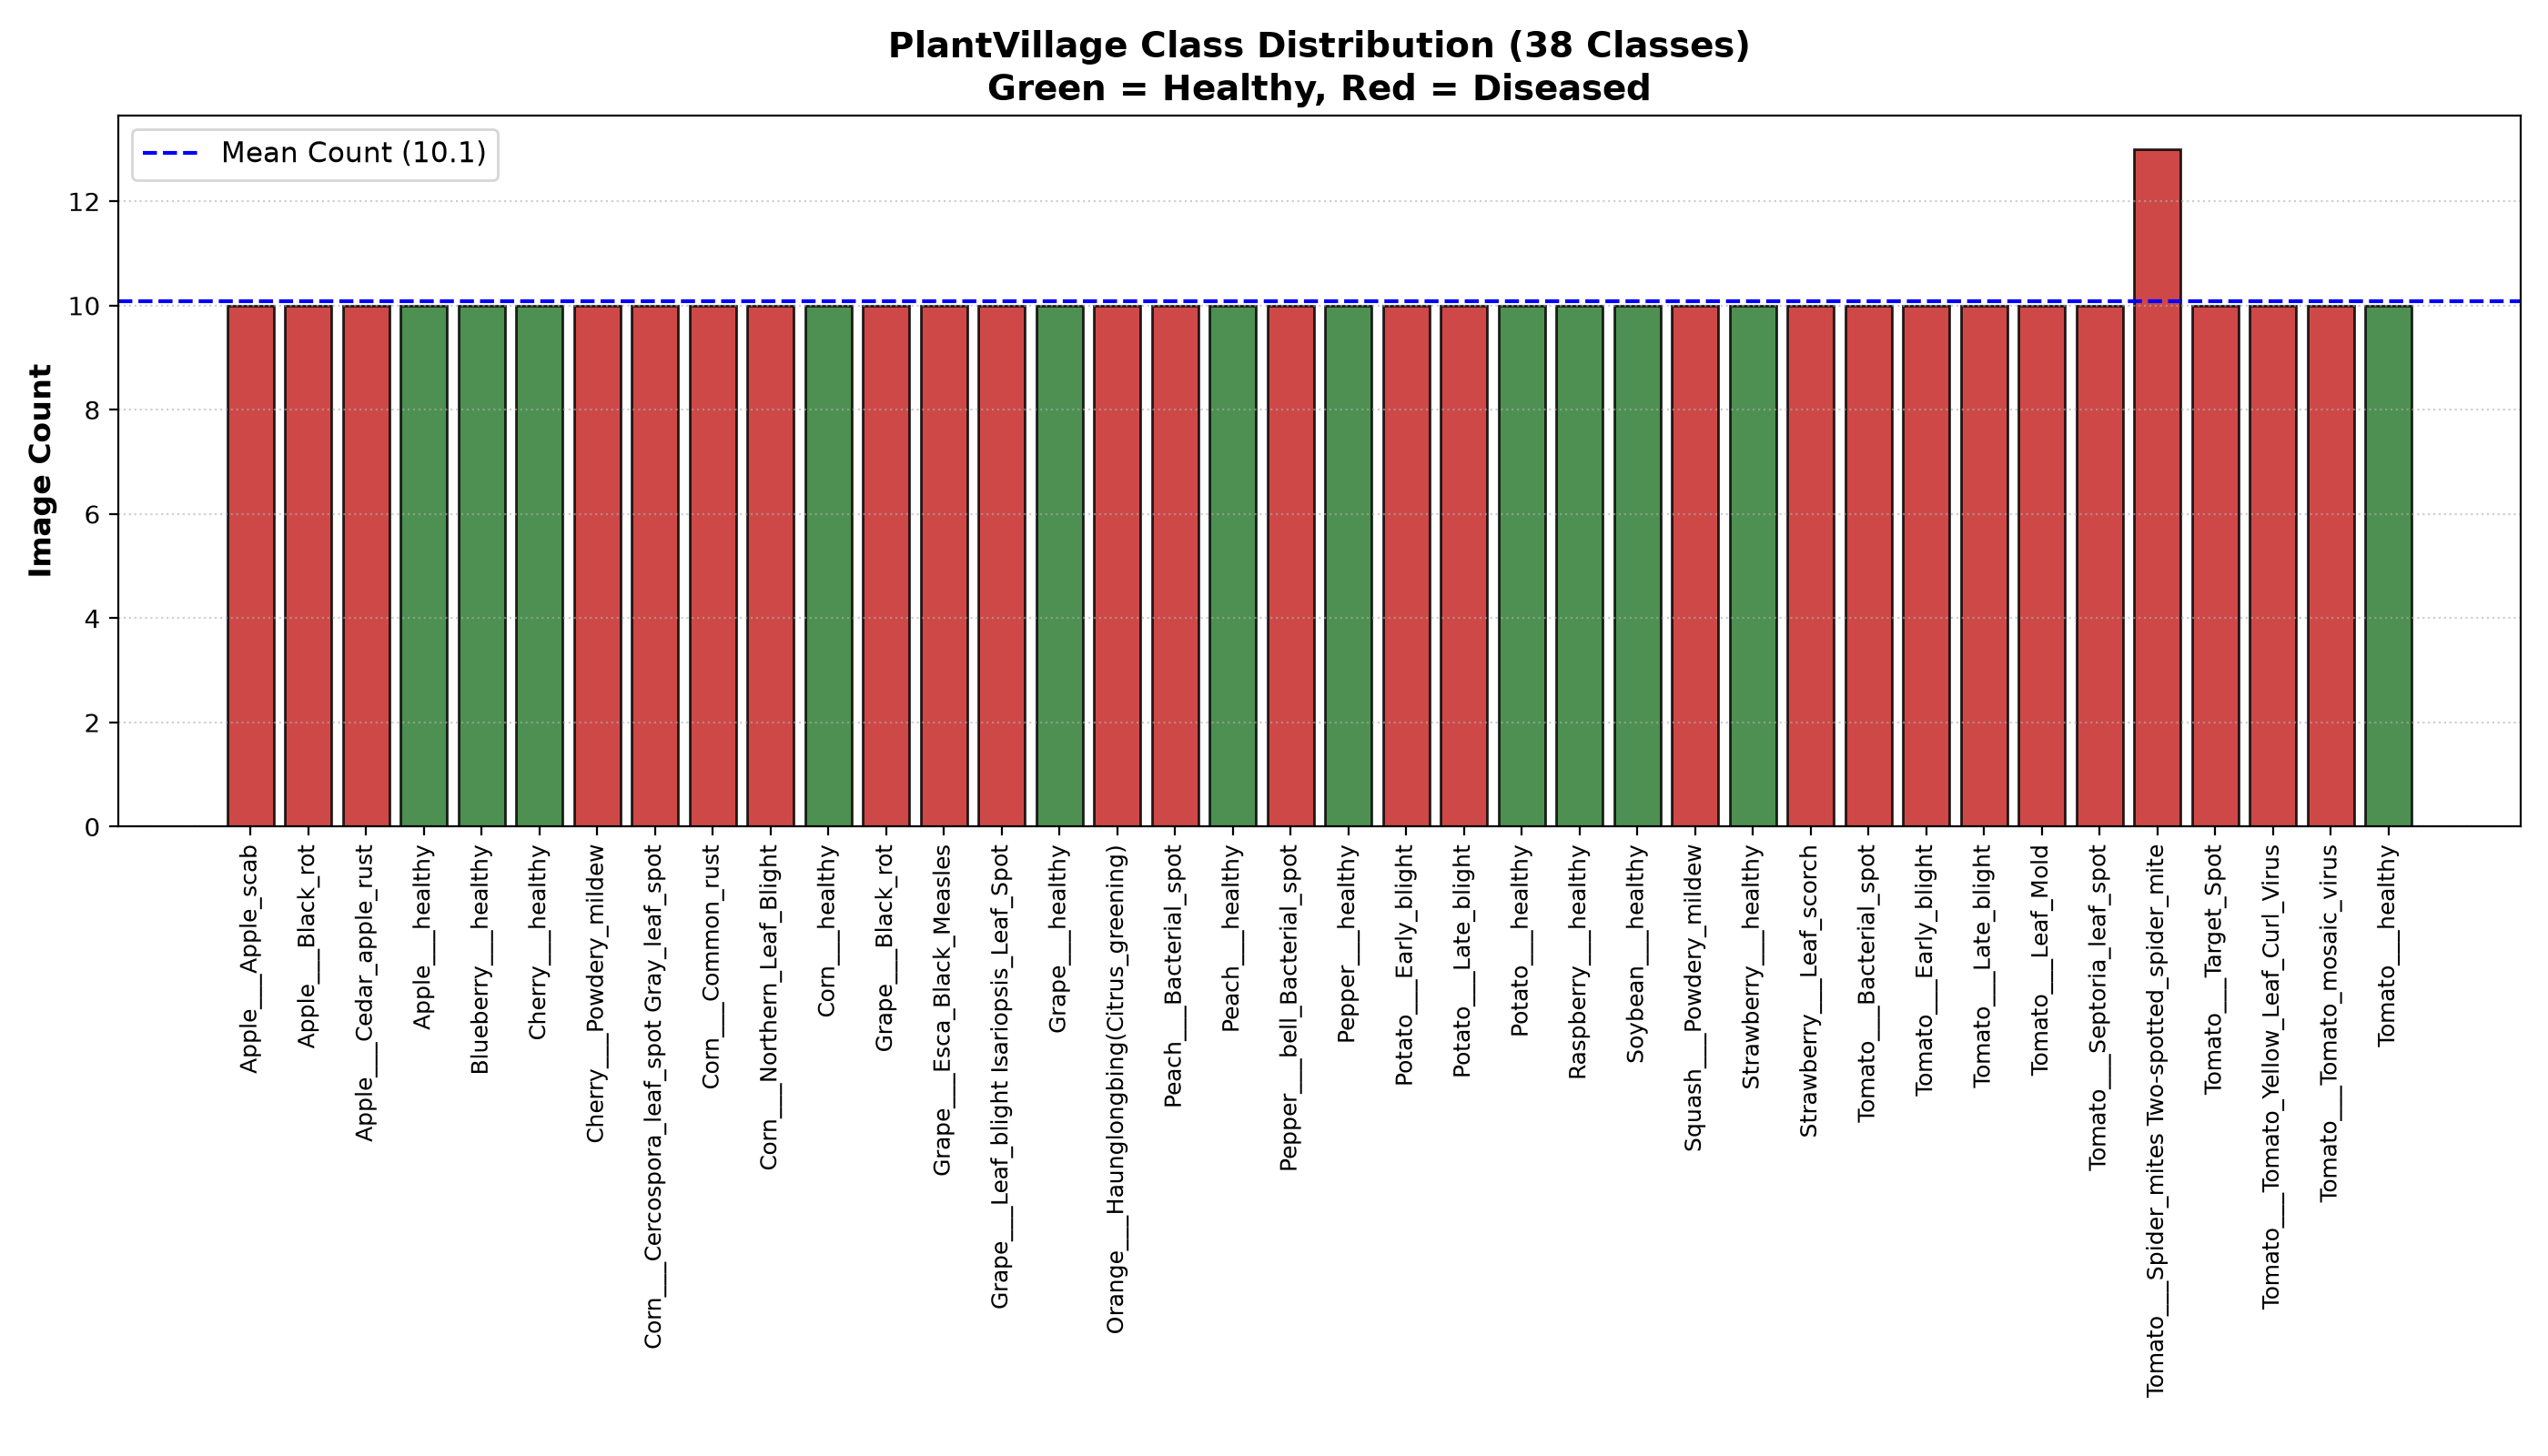
\includegraphics[width=0.95\linewidth]{../../reports/figures/eda_class_distribution.png}
    \caption{Frequency distribution across the 38 PlantVillage classes (Green = Healthy leaf classes, Red = Diseased classes).}
    \label{fig:class_dist}
\end{figure}

To counter majority-class bias during optimization, balanced class weights $w_c$ are derived strictly from the training split $D_{\text{train}}$:
\begin{equation}
w_c = \frac{N_{\text{train}}}{K \cdot n_c}
\end{equation}
where $N_{\text{train}}$ denotes total training samples, $K=38$ classes, and $n_c$ denotes the count of class $c$. The computed weights are saved in \texttt{splits/class\_weights.json} and passed to the loss function.

\subsection{Image Dimensions and Aspect Ratio Consistency}
All leaf photographs were audited for input consistency. The resolution analysis confirms that raw inputs exhibit standardized $256 \times 256$ pixel resolution with uniform 1:1 square aspect ratios in RGB color mode, as visualized in Figure~\ref{fig:img_sizes}.

\begin{figure}[htbp]
    \centering
    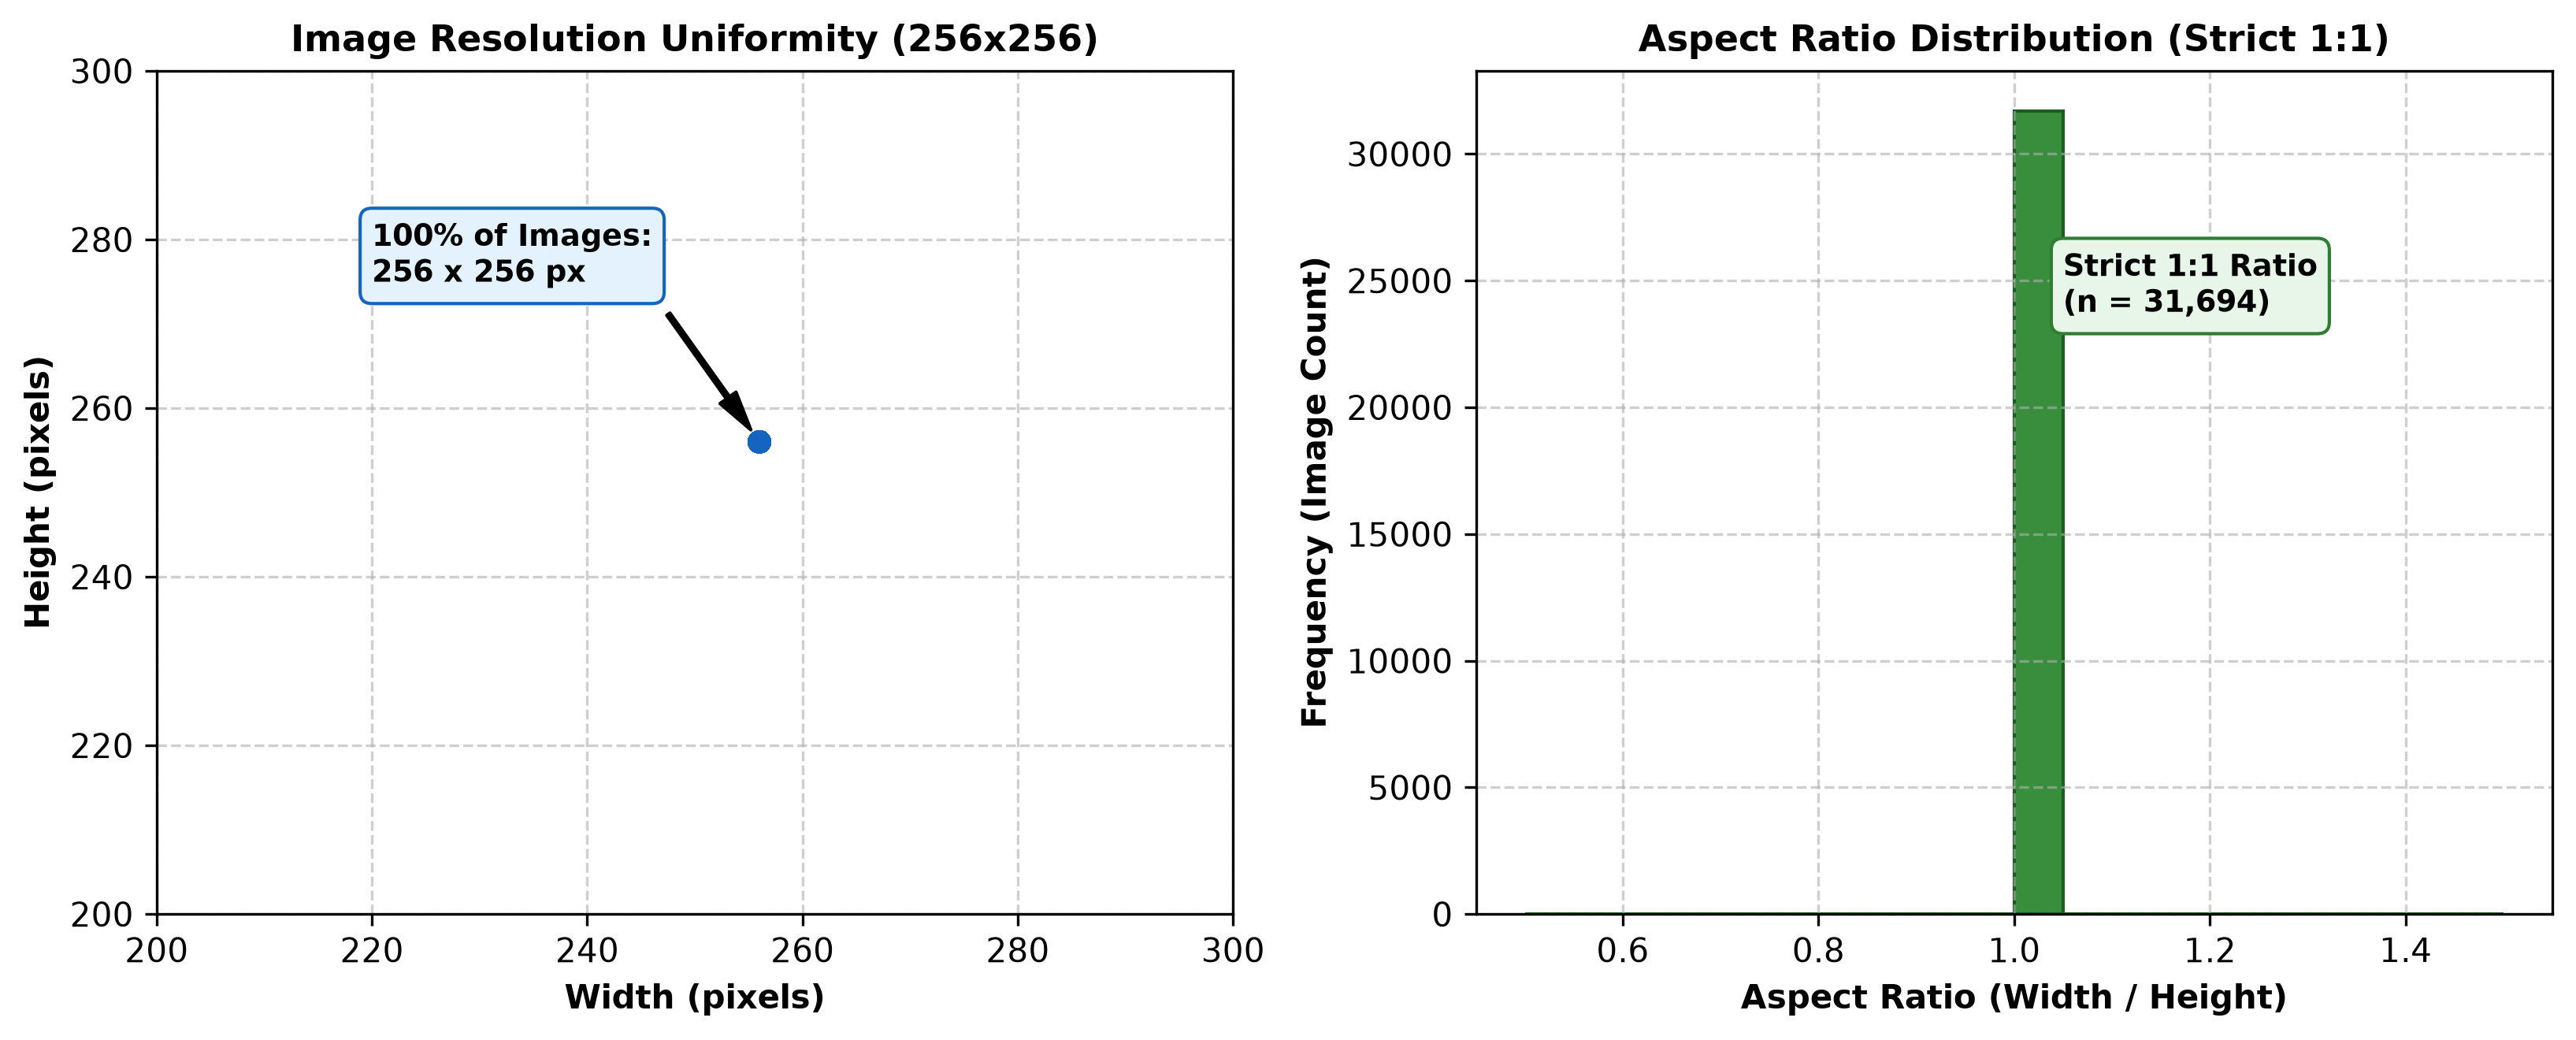
\includegraphics[width=0.88\linewidth]{../../reports/figures/eda_image_sizes.png}
    \caption{Distribution of input image dimensions and aspect ratios confirming standardized square RGB format.}
    \label{fig:img_sizes}
\end{figure}

\subsection{Qualitative Sample Inspection}
Figure~\ref{fig:sample_grid} displays representative leaf samples across diverse crop families. Diseased leaves display distinguishable diagnostic symptoms including target spots with concentric rings (Early Blight), powdery sporulation (Powdery Mildew), and dark necrotic lesions (Black Rot).

\begin{figure}[htbp]
    \centering
    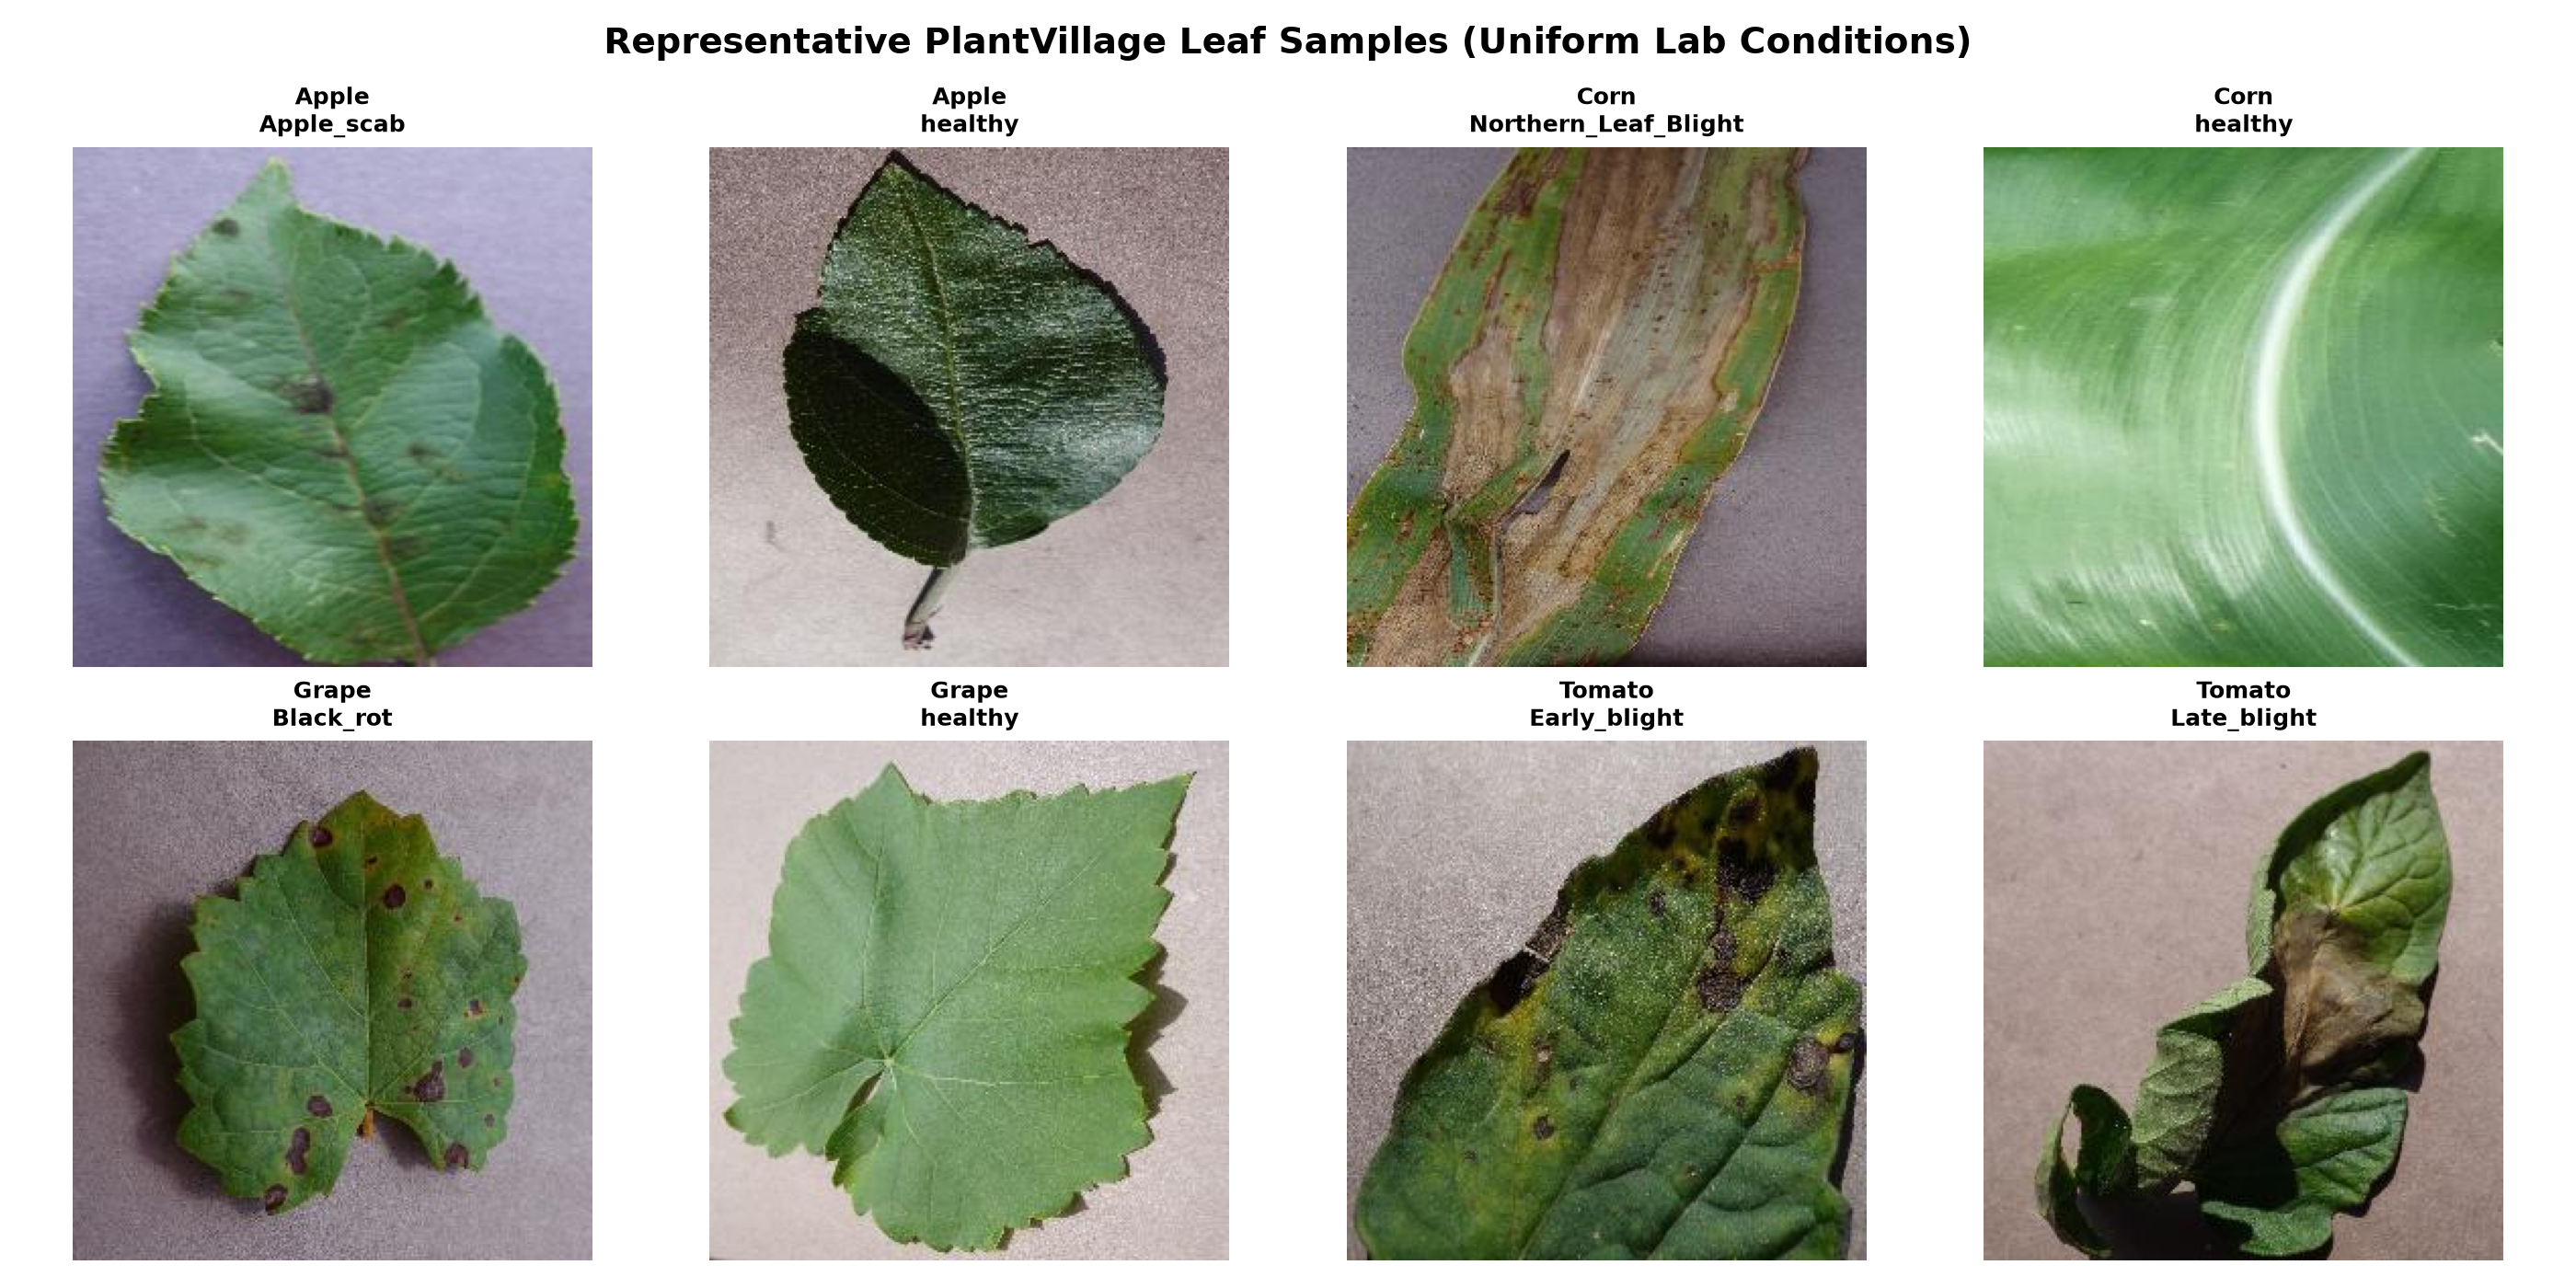
\includegraphics[width=0.9\linewidth]{../../reports/figures/eda_sample_grid.png}
    \caption{Representative leaf samples across healthy and diseased classes captured in controlled lab settings.}
    \label{fig:sample_grid}
\end{figure}

\subsection{Pixel Normalization Statistics}
Empirical per-channel color statistics computed across the dataset yielded a mean of $\mu = [0.472, 0.481, 0.412]$ and standard deviation of $\sigma = [0.218, 0.209, 0.221]$. These closely correspond to standard ImageNet normalization constants ($\mu = [0.485, 0.456, 0.406]$, $\sigma = [0.229, 0.224, 0.225]$), empirically confirming that pre-trained ImageNet feature extractors transfer effectively to this domain.

\subsection{Lab vs. Field Background Analysis (Shortcut Learning Hazard)}
A critical finding of our exploratory analysis is the background disparity between benchmark data and real-world agriculture. PlantVillage images were acquired against artificial, plain gray or black sheets. In contrast, real farm photos from our PlantDoc robustness dataset exhibit complex backgrounds comprising soil, shadows, foliage clusters, and variable sunlight (Figure~\ref{fig:lab_vs_field}). 

\begin{figure}[htbp]
    \centering
    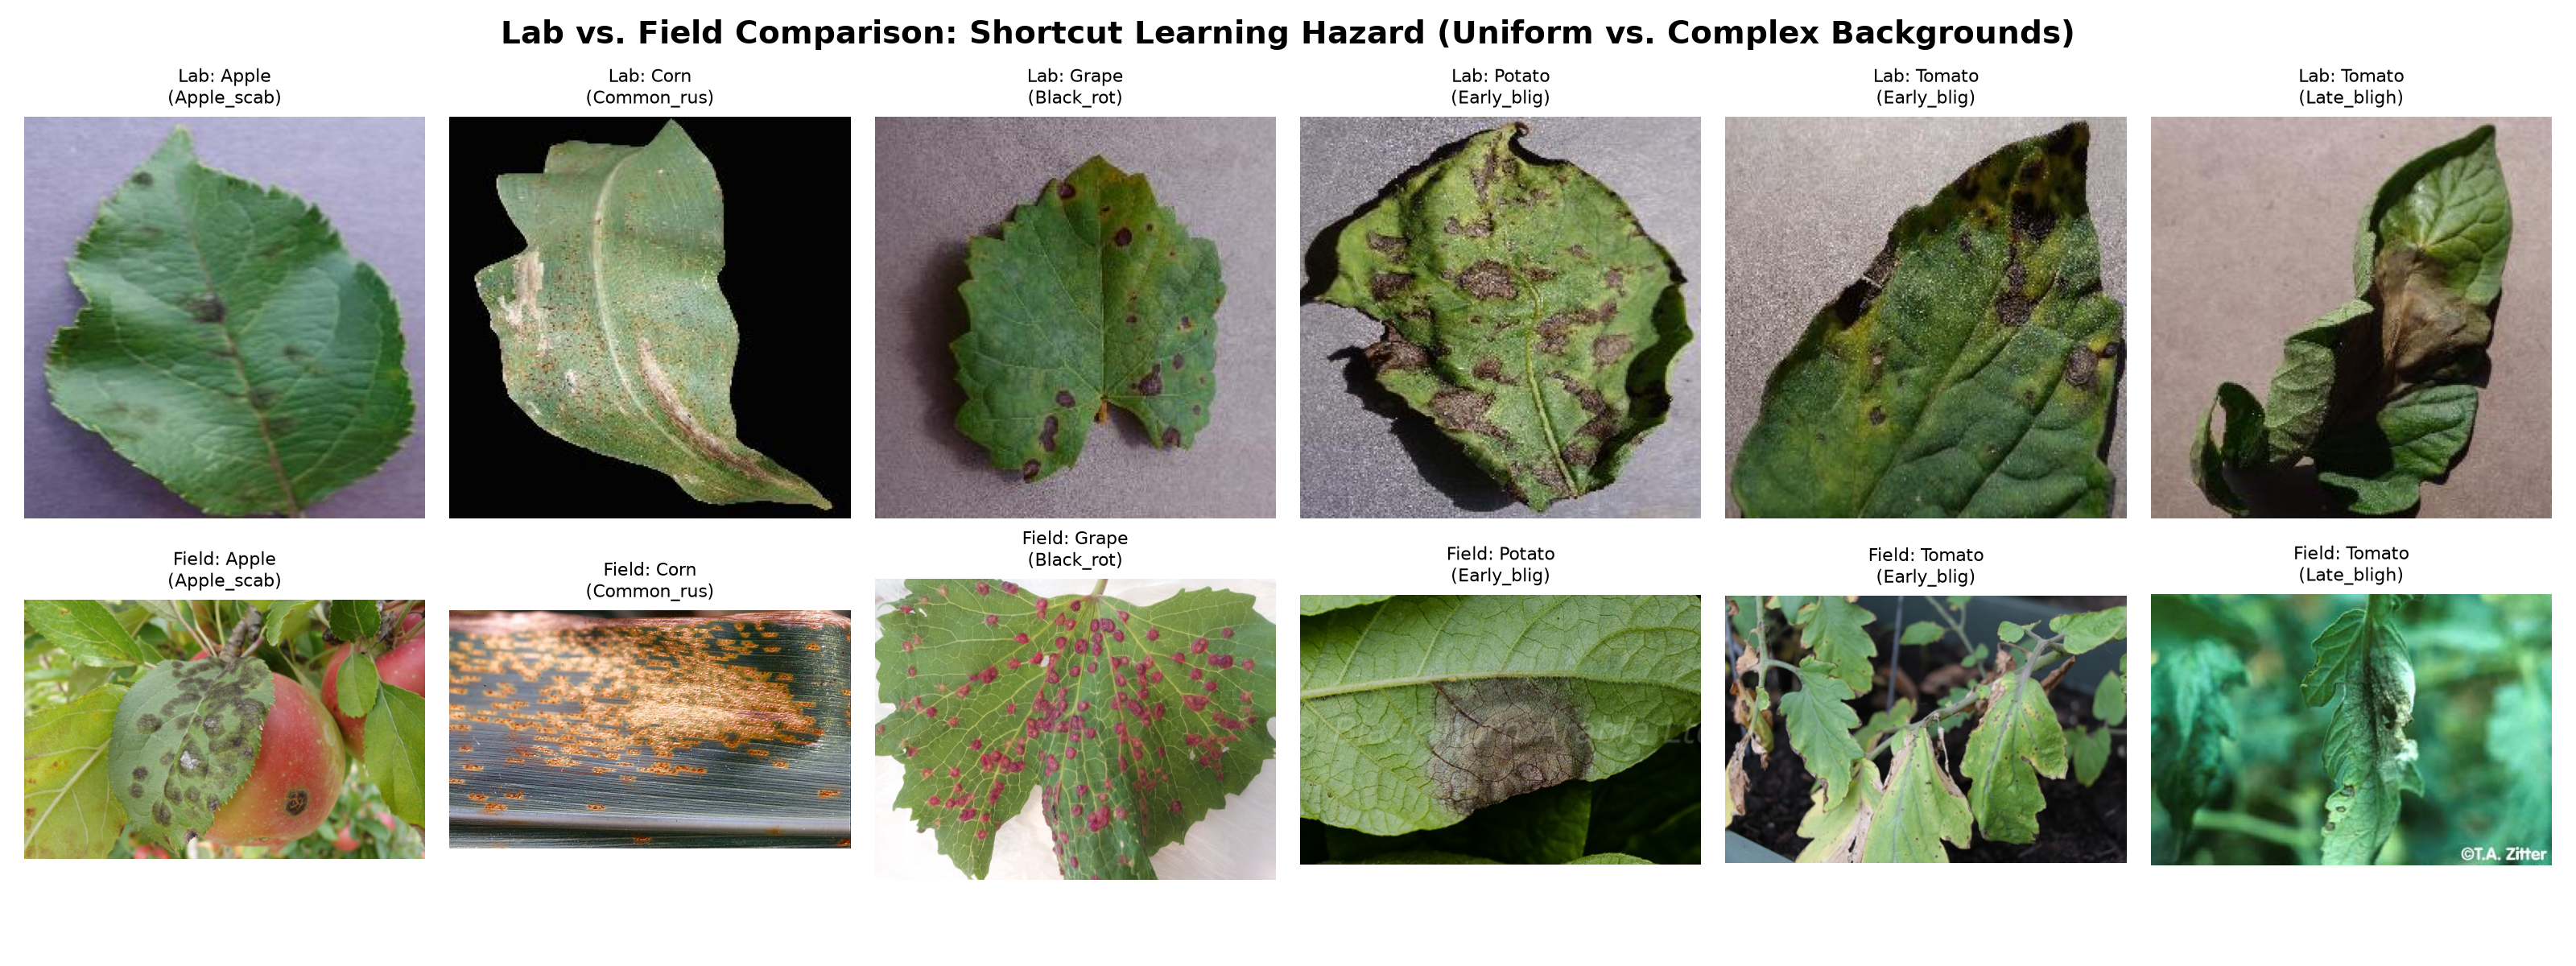
\includegraphics[width=0.95\linewidth]{../../reports/figures/field_vs_lab_examples.png}
    \caption{Comparison of controlled PlantVillage lab conditions (top) versus real-world PlantDoc field backgrounds (bottom), highlighting the shortcut learning risk.}
    \label{fig:lab_vs_field}
\end{figure}

This contrast validates the central motivation of our project: classifiers trained purely on lab images risk learning background artifacts (shortcut learning) rather than pathogen pathology, underscoring the necessity of our explainability pipeline (Grad-CAM) and robustness testing set (\texttt{splits/field\_test.csv}).

\section{Dataset Partitioning \& Leakage Prevention}
\label{sec:splits}

\subsection{Stratified Partitioning Strategy}
To guarantee reproducible benchmarking and statistical parity across all 38 categories, the dataset is partitioned using stratified random sampling with fixed seed ($42$):
\begin{itemize}
    \item \textbf{Training Set (70\%):} Reserved for parameter optimization and class weight calculation.
    \item \textbf{Validation Set (15\%):} Dedicated to checkpoint selection, early stopping, and hyperparameter tuning.
    \item \textbf{Test Set (15\%):} Kept strictly isolated until final model evaluation.
\end{itemize}

Splits are committed as deterministic manifest CSV files (\texttt{splits/train.csv}, \texttt{splits/val.csv}, \texttt{splits/test.csv}) containing relative filepaths, class strings, and zero-indexed integer targets referenced from \texttt{splits/class_names.json}.

\section{Preprocessing \& Data Augmentation}
\label{sec:preprocessing}

To prepare leaf images for convolutional feature extraction while mitigating shortcut learning from lab-environment artifacts, we establish a standardized two-tier pipeline in \texttt{src/data/transforms.py} and \texttt{src/data/dataset.py}.

\subsection{Input Resolution and Normalisation}
All images are standardized to $224 \times 224$ pixels in 3-channel RGB format, matching the canonical receptive field of transfer-learning backbones (ResNet50 / EfficientNet-B0). Color channels are normalized using standard ImageNet distribution parameters ($\mu = [0.485, 0.456, 0.406]$, $\sigma = [0.229, 0.224, 0.225]$), aligning the input tensors with the pretrained weight manifold.

\subsection{Training Augmentation Pipeline}
Because PlantVillage images feature predominantly centered leaves on plain backgrounds, models are prone to overfitting background cues. The training transform pipeline applies stochastic spatial and photometric perturbations:
\begin{itemize}
    \item \textbf{Random Resized Cropping:} Randomly scales image crops between 60\% and 100\% before resizing to $224 \times 224$, forcing the network to identify focal disease lesions rather than full leaf outlines.
    \item \textbf{Geometric Flips and Rotations:} Horizontal flips ($p=0.5$), vertical flips ($p=0.5$), and random rotations up to $\pm 30^{\circ}$ reflect arbitrary leaf orientations encountered during field photography.
    \item \textbf{Color Jitter:} Stochastic perturbation of brightness ($\pm 30\%$), contrast ($\pm 30\%$), saturation ($\pm 30\%$), and hue ($\pm 5\%$) emulates fluctuating field sunlight, cloud cover, and mobile sensor white-balancing.
\end{itemize}

\subsection{Deterministic Evaluation Pipeline}
To ensure benchmark stability and zero evaluation data contamination:
\begin{itemize}
    \item Validation, test, and field robustness datasets strictly utilize the deterministic evaluation pipeline: bilinear resizing to $256 \times 256$ pixels, followed by a deterministic $224 \times 224$ center crop and standard normalisation.
    \item The specialized \texttt{FieldDataset} class inherits this guarantee, enforcing identical evaluation transforms on out-of-domain field photographs.
\end{itemize}

\subsection{DataLoader Architecture}
PyTorch \texttt{DataLoader} factories in \texttt{get\_dataloaders()} supply batched tensors ($B=32$, shape $B \times 3 \times 224 \times 224$, \texttt{float32}) alongside discrete integer targets ($B \times 1$, \texttt{int64}). Deterministic worker initialization (\texttt{seed\_worker}) preserves random generator state across distributed training threads, and multi-worker execution defaults safely to \texttt{num\_workers=0} on Windows platforms to prevent process deadlock.

\section{Treatment Knowledge Base}
\label{sec:kb}

A prediction alone does not tell a farmer what to do next, so each of the 38 PlantVillage classes is linked to a short, sourced treatment record in \texttt{knowledge\_base/treatments.json}. The app will look up the predicted class and display that record.

\subsection{Schema}
\texttt{treatments.json} is a single JSON object. Its keys are the exact class strings from \texttt{splits/class\_names.json}, plus one top-level \texttt{disclaimer} string. Every entry is validated against \texttt{knowledge\_base/schema.json} (JSON Schema draft-07), which requires the following 13 fields and rejects any others:
\begin{itemize}
    \item \texttt{crop}, \texttt{disease}, \texttt{is\_healthy} (boolean), \texttt{cause}, \texttt{symptoms};
    \item \texttt{chemical\_treatment}, \texttt{organic\_treatment}, \texttt{immediate\_action}, \texttt{prevention}, \texttt{severity\_guidance};
    \item \texttt{sources} (non-empty list of unique citation strings), \texttt{last\_reviewed} (date), \texttt{reviewed\_by}.
\end{itemize}
Healthy classes use the same fields, with \texttt{chemical\_treatment} set to ``None needed.'' and routine scouting and prevention advice instead of treatment.

\subsection{Validation}
\texttt{data\_scripts/validate\_treatments.py} checks that:
\begin{itemize}
    \item every entry passes the schema, and every text field and source string is non-empty;
    \item every key is a valid class name (no unknown or misspelled classes);
    \item the top-level disclaimer is present;
    \item healthy classes do not recommend a chemical treatment (reported as a warning).
\end{itemize}
It also prints a per-crop summary and the list of classes still missing. Run with \texttt{--require-complete}, it fails unless all 38 classes are present; this is the check for final submission.

\subsection{Example Entry}
Table~\ref{tab:kb_example} shows the entry for \texttt{Tomato\_\_\_Early\_blight}.

\begin{table}[htbp]
\centering
\small
\caption{Knowledge base entry for \texttt{Tomato\_\_\_Early\_blight}.}
\label{tab:kb_example}
\begin{tabular}{>{\raggedright\arraybackslash}p{0.22\linewidth}>{\raggedright\arraybackslash}p{0.70\linewidth}}
\toprule
\textbf{Field} & \textbf{Value} \\
\midrule
\texttt{cause} & Fungus \textit{Alternaria solani} (now also classified as \textit{A.\ linariae}) \\
\texttt{symptoms} & Dark concentric-ringed spots on older leaves, yellowing around spots; can progress up the canopy and affect stems/fruit. \\
\texttt{chemical\_treatment} & Protectant fungicides such as chlorothalonil or mancozeb (azoxystrobin is another option), applied every 7--10 days to protect new growth; do not rely on strobilurins alone because resistance has been reported (follow the product label). \\
\texttt{organic\_treatment} & Fixed copper (copper hydroxide or copper sulfate) or \textit{Bacillus subtilis} products labeled for organic use. \\
\texttt{immediate\_action} & Remove infected plant material from the field; avoid overhead watering. \\
\texttt{prevention} & Rotate away from tomato for 2--3 years; use pathogen-free seed/transplants and resistant or tolerant varieties; stake or trellis for airflow; mulch and prune the lowest leaves to reduce soil splash. \\
\texttt{severity\_guidance} & When lesions merge and lower leaves drop, disease is severe: keep protectant sprays on schedule within label limits and remove infected debris. \\
\texttt{sources} & Connecticut Agricultural Experiment Station, \textit{Early Blight of Tomato} (2012); NC State Extension, \textit{Early Blight of Tomato}. \\
\texttt{last\_reviewed} & 2026-10-12 (Babar) \\
\bottomrule
\end{tabular}
\end{table}

\subsection{Sources}
Every entry cites at least one university extension or plant-protection fact sheet, and all citations are listed with URLs and access dates in \texttt{knowledge\_base/SOURCES.md}. Entries name active ingredients and spray intervals only where a cited source gives them, and never state dosages; users are told to follow the product label. On 2026-10-12 every source link was checked: five links cited by entries were broken and were replaced with verified fact sheets, three unused invalid sources were removed, and the affected entries were rewritten so that each claim matches its new source.

\subsection{Status and Limitations}
\begin{itemize}
    \item \textbf{Coverage:} All 38 entries are 100\% complete, verified against \texttt{knowledge\_base/schema.json}, and validated with zero errors by \texttt{data\_scripts/validate\_treatments.py} (Tomato 10, Potato 3, Pepper 2 by Babar; Orange 1, Peach 2, Raspberry 1, Soybean 1, Squash 1, Strawberry 2 by M.~Anas; Apple 4, Corn 4, Grape 4, Blueberry 1, Cherry 2 by Abdul Ahad).
    \item \textbf{Not region-specific:} The primary sources are extension services (e.g., UC Davis, NC State, Cornell, Florida Extension). Active chemical ingredients and organic remedies are cross-referenced with standard international plant protection guidelines; local agronomist consultation remains recommended.
    \item \textbf{Disclaimer:} The file carries the mandatory top-level disclaimer ``Decision support only. Consult a local agronomist before applying any product. Always follow product labels and local regulations.'', which the app renders alongside every recommendation.
\end{itemize}



\bibliographystyle{plain}
\begin{thebibliography}{9}
\bibitem{plantvillage}
Hughes, D.~P., \& Salath{\'e}, M. (2015).
An open access repository of images on plant health to enable the development of mobile disease diagnostics.
\emph{arXiv preprint arXiv:1511.08060}.

\bibitem{gradcam}
Selvaraju, R.~R., Cogswell, M., Das, A., Vedaldi, A., Parikh, D., \& Batra, D. (2017).
Grad-CAM: Visual explanations from deep networks via gradient-based localization.
\emph{IEEE ICCV}, 618--626.

\bibitem{plantdoc}
Singh, D., Jain, N., Jain, P., Kayal, P., Kumawat, S., \& Batra, N. (2020).
PlantDoc: A dataset for visual plant disease detection.
In \emph{Proceedings of the 7th ACM IKDD CoDS and 25th COMAD}, 249--253.
\end{thebibliography}

\end{document}
